\chapter{Sound Event Localization and Detection}
\label{chap:seld2019}


%%%%%%%%%%%%%%%%%%%%%%%%%%%%%%%%%%%%%%%%%%%%%%%%%%%%%%%%%%%%
%%%%%%%%%%%%%%%%%%%%%%%%%%%%%%%%%%%%%%%%%%%%%%%%%%%%%%%%%%%%
\section{Introduction}
\label{sec:intro}
%


Sound Event Localization and Detection (SELD) refers to the problem of identifying, for each individual event present in a sound field, the \textbf{spatial location} $\Omega$, \textbf{temporal activity} $\Upsilon$, and \textbf{sound class} $\kappa$ to which it belongs. 

The organization of a dedicated SELD task within the IEEE AASP Challenge on Detection and Classification of Acoustic Scenes and Events (DCASE) 2019 can be considered as a milestone for the development of the SELD research problem. 
Indeed, a large number of novel methodologies were developed for the Challenge, most of them based on Convolutional Recurrent Neural Networks (CRNN). The performance of the baseline method, a CRNN that performed jointly the localization and classification tasks \cite{Adavanne2018_JSTSP}, was vastly exceeded by a variety of deep-learning based algorithms \cite{kapka2019sound, Cao2019, grondin2019sound}.
Some of these improvements have been included in the baseline system for the SELD Challenge of DCASE 2020. \\

Despite the predominant trend towards high-complexity deep-learning architectures, some recent works have been able to match or even improve CRNN-based methods with regard to localization, by using parametric analysis of the ambisonic sound field \cite{perez2019hybrid, nguyen2020sequence}.  
Apart from the benefit derived by their simplicity, these approaches are able to resolve the case of overlapping events of the same class, a situation difficult to disambiguate for CRNN-based methods \cite{politis2020dataset}.\\


The present work continues the exploration of possibilities of parametric SELD methods, focusing on a low-complexity architecture that makes use of traditional, feature-based machine learning techniques. The method has been developed in the context of the SELD task within DCASE 2020 Challenge, and therefore utilizes the proposed dataset, baseline system and evaluation metrics.\\

Finally, it is important to remark that the method described here is the continuation of an algorithm presented at the DCASE 2019 Challenge \cite{perez2019hybrid}; both algorithms share a common structure and a similar approach to the SELD problem. 
However, the current proposal tries to solve some of the problems identified on our early approach, mainly related with a low frame recall derived from a naive approach to event segmentation. Moreover, the current method also presents a complexity reduction, regarding the single-source 
DOA estimation and the classifier. 


\newpage
%%%%%%%%%%%%%%%%%%%%%%%%%%%%%%%%%%%%%%%%%%%%%%%%%%%%%%%%%%%%
%%%%%%%%%%%%%%%%%%%%%%%%%%%%%%%%%%%%%%%%%%%%%%%%%%%%%%%%%%%%
\section{System description}
\label{sec:methodology}

The proposed method, referred to as \textit{PAPAFIL}, can be summed up in four steps:

\begin{enumerate}
    \item Estimate single-source time-frequency bins.
    \item Use a particle tracking system to estimate event trajectories and activation times from single-source bins.
    \item Perform spatio-temporal filtering on the input signal.
    \item Assign a class label to the estimated event.
    % \item The estimated event is assigned a class label by a classifier.
\end{enumerate}

A scheme of the method is shown in Fig.~\ref{fig:scheme}.

\begin{figure}[th!]
  \centering
  \centerline{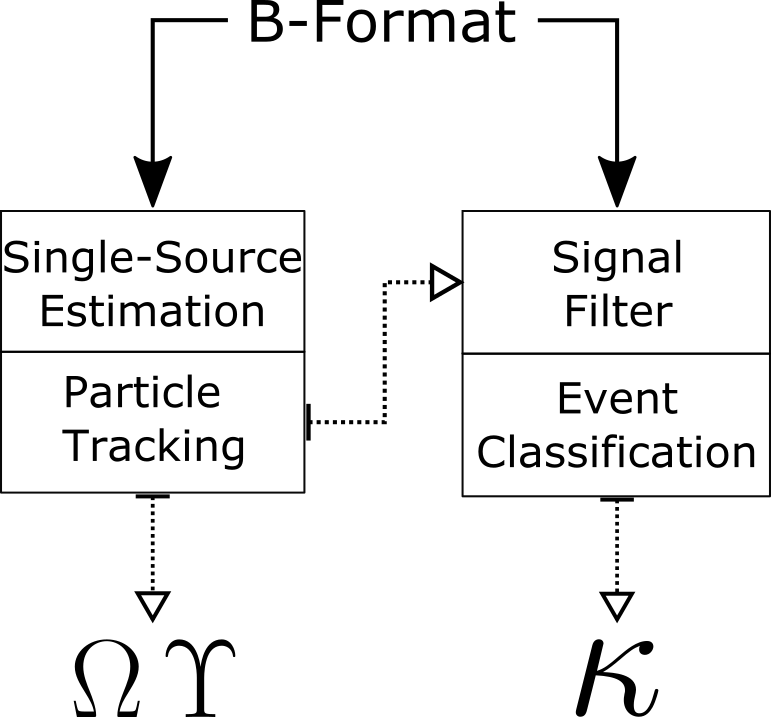
\includegraphics[width=0.55\textwidth]{Figures/SELD/ARCH.png}}
  \caption{Architecture of the proposed methodology.}
  \label{fig:scheme}
\end{figure}


%%%%%%%%%%%%%%%%%%%%%%%%%%%%%%
\subsection{Single-source estimation}

The first step is the transformation of the B-Format input signal $x_n^m(t)$ using the Short-Time Fourier Transform (STFT) into the time-frequency (TF) signal $X_n^m(k,n)$.

In the resulting spectrogram, the frequencies above a given limit $f_{max}$ are discarded; this procedure speeds up the method while maintaining the directional information, given that the microphone geometry produces spatial aliasing above approx. 5 kHz \cite{Bertet2006}.

Assuming that the sources are sparse in time-frequency, it could be possible to identify TF bins which contain a significant energetic contribution from only one source.
% i.e., without significant cross-talk from other sources or background noise. 
These bins could be then used to produce accurate DOA estimates. The effectiveness of this approach has already been demonstrated \cite{tho2014robust, nguyen2020sequence}.

Single-source TF bins are computed from the DirAC parametric analysis.
A variety of alternative subspace methods are known \cite{epain2016spherical, madmoni2018direction}; however, those methods require local estimation of eigenvalues through the Spatial Covariance Matrix (SCM), which is a computationally expensive procedure;
this is the main reason for the choice of DirAC-based analysis in this work. 

A TF bin is counted as single-source if its diffuseness $\Psi(k,n)$ is lower than a threshold $\Psi_{max}$. Diffuseness is computed here using Eq.~\ref{eq:psidefinition}. 
 Finally, the DOA $\Omega(k,n)$ of the TF bins passing the aforementioned single-source test is computed as the angle of the active intensity vector by Eq.~\ref{eq:doa}.
 To illustrate the process, an example of the method output is plotted in Fig.~\ref{fig:plots} (top).
% As an example, Fig.~\ref{fig:plots} (top) plots the estimated DOAs of single-source TF bins.

\begin{figure}[th!]
  \centering
  \centerline{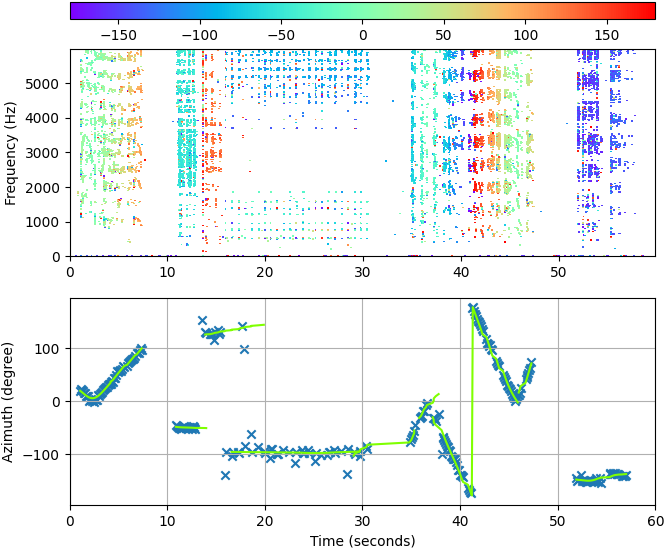
\includegraphics[width=\columnwidth]{Figures/SELD/plots.png}}
  \caption{Estimation of localization and temporal activation. Top: azimuth spectrogram after diffuseness mask; color indicates estimated position of a TF bin passing the single-source test. Bottom: input/output of the particle tracking; the crosses represent the measurement space, and the continuous lines are the resulting events.}
  \label{fig:plots}
\end{figure}

 

%%%%%%%%%%%%%%%%%%%%%%%%%%%%%%
\subsection{Particle tracking}

Once a set of reliable TF DOA estimates is obtained, the next step is the generalization of the individual measurements into trajectories and temporal activations.
% Given that the instantaneous number of sources is unknown, it is necessary to use a multiple target tracker. 
In our case, we opted for the Rao-Blackwellized Monte-Carlo Data Association (RBMCDA) algorithm \cite{sarkka2004rao}, which decomposes the multiple target tracking problem in two: it solves first the data association problem, and then performs the single target tracking individually. 
This method has been recently used in the context of sound event localization and tracking with successful results \cite{Adavanne2018_JSTSP, adavanne2019localization}; the code used for our implementation has been adapted from the same authors\footnote{\url{https://github.com/sharathadavanne/multiple-target-tracking}}.

The system takes as the input the set of TF DOA values passing the single source test, and produces spatio-temporal event trajectories, considering an event as an entity with contiguous temporal activation and continuous spatial position. 
More specifically, for each time frame, the median\footnote{Circular median in the case of azimuth.} of all narrowband masked DOA estimates is computed. The resulting value is added to the measurement space of the tracker if the number of single-source frequency bins for that frame exceeds a minimum $K_{min}$. 

The performance of the RBMCDA algorithm is controlled by several parameters. Some of the most relevant ones are the angular velocity prior $v$, the standard deviation $\sigma_{\nu}$ and the spectral density $s_{\nu}$ of the measurement noise, the prior probabilities of birth $p_{birth}$ and noise percentage $p_{\nu}$, and the number of Monte-Carlo particles $N$. Position-related parameters are adjusted with respect to their ranges, so that azimuth-related magnitudes double elevation values.  



The procedure is followed by a numerical post-processing step, which includes data interpolation, resampling (if needed), and removal of elements shorter than $T_{min}$.
Finally, the system provides a list of $J$ events, each one having an instantaneous position $\Omega_j(t)$ and a temporal activation $\Upsilon_j$. 
An example of the system inputs and outputs is depicted in Fig.~\ref{fig:plots} (bottom).



 
%%%%%%%%%%%%%%%%%%%%%%%%%%%%%%
\subsection{Signal filter}

The information provided by the particle tracking system is used to spatially filter the input signal. This can provide an enhanced monophonic estimate of an event $\tilde{s}_j(t)$ with reduced influence of simultaneous events.
The process is performed by steering a virtual first-order cardioid in the direction of interest, using Eq.~\ref{eq:decoding}.
%\begin{equation}
%	\tilde{s}_j(t) = \sum_{m=0}^{M-1} x_m(t) Y_m(\Omega_j) \alpha_n
%	\label{eq:decoding}
%\end{equation}
%where $\bm{Y}(\Omega_j) = [Y_0(\Omega_j), \dots, Y_3(\Omega_j)]^\intercal$ are the real-valued spherical harmonics up to first order evaluated in the direction $\Omega_j$ \cite{daniel2000representation}, and the column vector $\alpha_n$ controls the beam pattern directivity.
 The result of this process is a monophonic estimate for each event, $\tilde{s}_j(t)$, temporally delimited by $\Upsilon_j$. 
 As a last step, each estimate is amplitude peak-normalized, in order to minimize potential amplitude variability due to arbitrary configurations of the scene. 


%%%%%%%%%%%%%%%%%%%%%%%%%%%%%%
\subsection{Event classification}
As a final step, a class label is assigned to each estimated event $\tilde{s}_j(t)$ using a single-class classifier. Since the objective is to keep complexity low and make results interpretable, a machine learning algorithm is used instead of deep learning frameworks. The main advantages of this choice are: (i) low number of parameters; (ii) low train and predict computational time, easing reproducibility; and (iii) relative importance of the features in the output can be interpreted, which is not possible with deep learning approaches.

Gradient Boosting Machine (GBM, Fig.~\ref{fig:gbm}) has been selected as the classification algorithm since it is a powerful yet simple technique for predictive modeling. 
In essence, the algorithm is aimed to minimize the loss of the objective function by adding many weak learners. These learners are typically simple decision trees and their parameters are tuned using gradient descent techniques. 
GBM implementation makes use of the \textit{scikit-learn} library \cite{scikit-learn}.
% Specifically, XGBoost framework is implemented for training process due to its proven performance in a wide range of classification problems \cite{xgboost}.

\begin{figure}[t]
  \centering
  \centerline{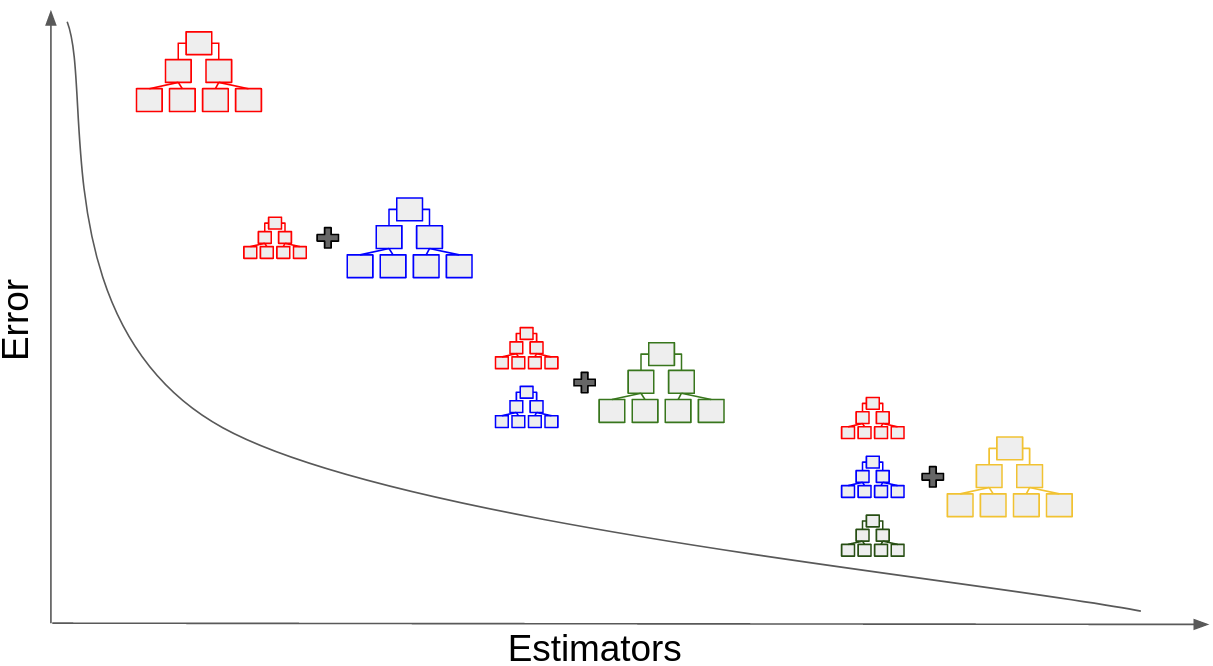
\includegraphics[width=0.75\columnwidth]{Figures/SELD/gbm.png}}
  \caption{Gradient boosting machine learning process. Adding weak estimators allows reducing overall error in the predictions.}
  \label{fig:gbm}
\end{figure}

Sound features are obtained using extractors from \textit{Essentia}, an open-source library for audio analysis \cite{bogdanov2013essentia}. 
Given the heterogeneous nature of the sound classes, a mixture of spectral, temporal and harmonic features are used, as shown in Table~\ref{tab:features}. 
Features are be computed either frame-based or on the whole event; in the former case, the classifier is fed with their temporal first-order statistics. 
% This is the situation for all \textit{Low-level}, and some \textit{SFX} features.
% Conversely, event-level features are passed directly to the classifier. 



\begin{table}[t!]
\caption{Acoustic features used for classification, grouped by type.}
\begin{footnotesize}
\begin{center}
\begin{tabular}{ccc}
\toprule
Type & Features & Number \\
\midrule
\textit{Low-level} & Mel bands & 24       \\
& MFCC & 13 \\
& Spectral Features & 26 \\
% & Pitch Salience &1 \\
\midrule
% SFX & Total and perceived&2 \\
% & sound duration & \\
% & Descriptors based on pitch & 4 \\
% & and harmonics estimation & \\
% & Sound envelope descriptors & 11\\
% & Pitch envelope descriptors & 4\\
\textit{SFX }& Duration &2 \\
& Harmonic & 4 \\
& Sound envelope & 11\\
& Pitch envelope & 4\\
\bottomrule
\end{tabular}
\end{center}
\end{footnotesize}
\label{tab:features}
\end{table}



%%%%%%%%%%%%%%%%%%%%%%%%%%%%%%%%%%%%%%%%%%%%%%%%%%%%%%%%%%%%
%%%%%%%%%%%%%%%%%%%%%%%%%%%%%%%%%%%%%%%%%%%%%%%%%%%%%%%%%%%%

\section{Experiments}
\label{sec:experiments}


\subsection{Dataset and baseline system}

The dataset used is the FOA subset of the development set of the \textit{TAU-NIGENS Spatial Sound Events 2020} \cite{politis2020dataset}, which features 600 different B-Format clips of 60 seconds long each. 
Each clip contains multiple sound events, which belong to one of the fourteen sound classes from the NIGENS database \cite{trowitzsch2019nigens}.
Events are also located at a potentially time-varying positions, and the maximum instantaneous overlapping of sources allowed is limited to two. Fifteen different Room Impulse Responses (RIR) are used for scene reverberation, covering a vast range of acoustic conditions. Furthermore, the audio clips contain a moderate amount of recorded background sounds. 

The baseline method is based on the recently proposed SELDnet architecture  \cite{Adavanne2018_JSTSP}, which features a Convolutional Recurrent Neural Network (CRNN) that solves both localization and classification problems jointly. 
Additionally, the baseline implementation has been improved with several changes inspired by one of the best performing methods in DCASE 2019 Task 3 Challenge \cite{Cao2019}. 

\subsection{Experimental setup}


In order to explore the performance of the system, two different approaches have been undertaken regarding the creation of the training dataset for the monophonic single-class classifier. 
The first approach, referred to as \textit{PAPAFIL1}, collects all event localization, temporal activation and class information by parsing the annotation files.
Conversely, the second approach, called \textit{PAPAFIL2}, uses the proposed parametric particle filter to estimate localizations and activations, and the class label is assigned to each event by a custom association algorithm based on spatio-temporal distance. 
In both cases, the input signal is filtered with the obtained information in order to conform the monophonic event estimates.

Therefore, the difference between training datasets is noticeable: while the training events in \textit{PAPAFIL1} are more accurately determined than in \textit{PAPAFIL2}, the differences with respect to the prediction scenario are much bigger in the former case. 
% Consequently, a slightly better performance of the second method might be expected, provided that the parametric particle filter performance has some degree of robustness and accuracy.
The number of individual events for each of the approaches is plotted in Fig.~\ref{fig:num_events}. Approximately half of the classes have similar number of instances in both datasets. However, the other half presents noticeable differences, which might be explained by the different criteria applied for the consideration of event temporal activations: the groundtruth seems to follow a frame-based activity detection approach, while the output of the proposed method tends to consider events as time-continuous manifestations, influenced by the particle filter.

This situation leads to two different \textit{oracle} systems (referred to by appending \textit{-O} in the method name), which represent the best performance theoretically achievable for the corresponding method. 

\begin{figure}[t]
  \centering
  \centerline{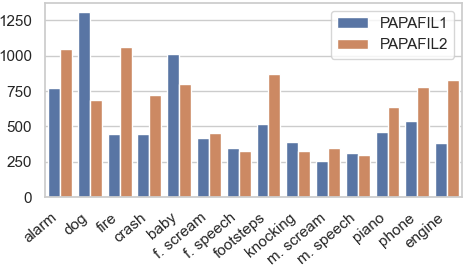
\includegraphics[width=\columnwidth]{Figures/SELD/numclasses2_tight.png}}
  \caption{Number of occurrences of each event class in the training set, for both proposed methods. }
  \label{fig:num_events}
\end{figure}


The accurate information of the \textit{PAPAFIL1} training set suggests a need for data augmentation; 
in contrast, the training material used in \textit{PAPAFIL2} is already provided by a certain extent of variability.
This situation motivates the implementation of data augmentation methods in the \textit{PAPAFIL1} training set.
Specifically, several standard data augmentation techniques are implemented: pitch shifting, time shifting, time stretching and white noise addition.
Furthermore, given the observed high influence of reverberation in the system performance, a reverberant data augmentation technique based on synthetic RIRs has been considered. 
Ten different single-channel RIRs, with reverberation times between 0.3 and 1.1 seconds, have been synthetically created using the \textit{masp} library \cite{perez2020python}. During training, each event estimate is convolved with one of the RIRs, randomly chosen. 
RIR augmentation has recently been shown very effective for blind reverberation time estimation \cite{bryan2020impulse} but, to the best of the authors' knowledge, this is the first application in SELD.

% The presented scheme leads to two different \textit{oracle} systems (named by an \textit{-O} appendix in the method name), which represent the best performance theoretically achievable for the corresponding method. 

% In this way, it is expected that \textit{PAPAFIL1-O} obtains very high localization scores overall, while the performance of \textit{PAPAFIL2-O} can be much similar to the non-oracle case.

% It is important to notice that the spatial filtering is performed with a first-order cardioid, which provides a broad directive pattern. Accordingly, in the case of overlapping events, there will be always signal cross-talk, even when using the groundtruth annotations. The usage of higher ambisonic orders could easily mitigate this effect. 

Table~\ref{tab:parameter} shows a comprehensive list of the parameters used throughout the different steps of the proposed method. All values are equal for both presented approaches, except for the number of Monte-Carlo particles $N$. 
The values for Single-Source Estimation and Particle Filtering parameters have been iteratively refined by manual tuning and inspection, departing from standard values. 
The beamforming weights $\alpha_m$ correspond to the \textit{maximum directivity beamformer}, which minimizes the energy contributions from directions other than the lookup direction \cite{rafaely2015fundamentals}. In the spatial audio field, such property is also known as the \textit{max-rE} decoder \cite{daniel2000representation}. 
Regarding event classification, a cross-validation scheme has been implemented for tuning GBM hyperparameters. 
% In addition, unlike other methods such as CRNN, GBM allows to analyze the relative importance of each feature in the classifier. As it can be seen in Figure \ref{fig:importance}, the most representative variable is sfx.duration, being also important lowlevel.mfcc and spectral variables.

% \begin{figure}[t]
%   \centering
%   \centerline{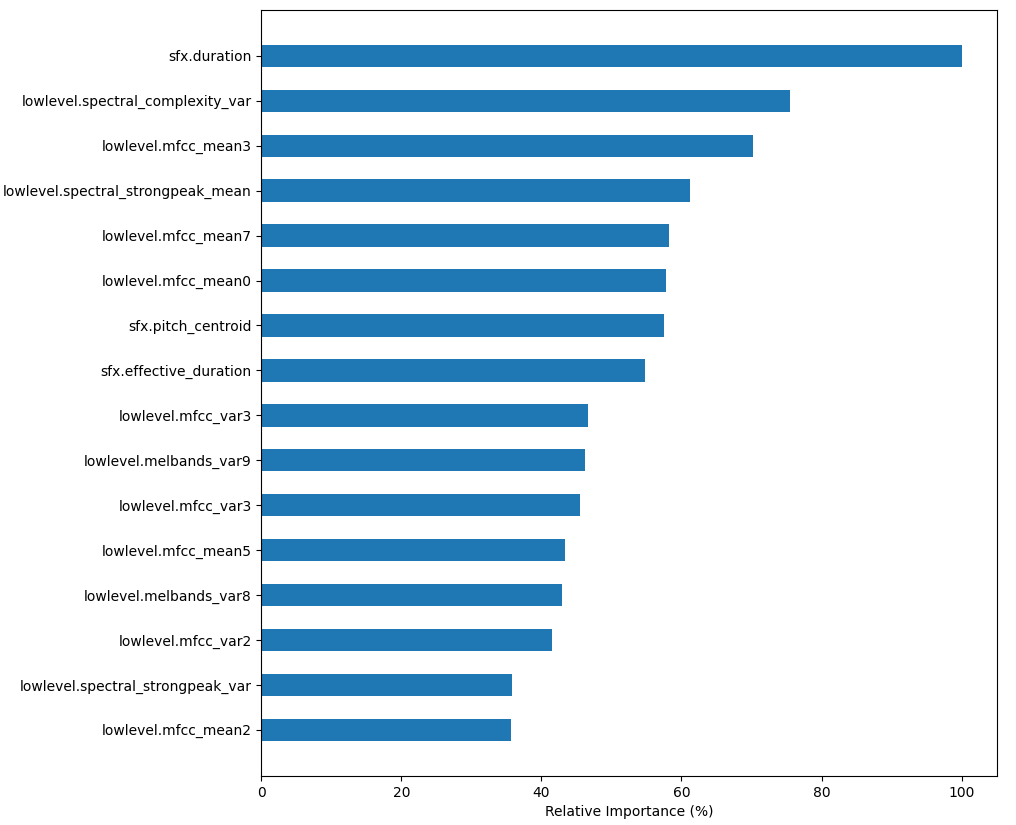
\includegraphics[width=1\columnwidth]{Figure_2.png}}
%   \caption{Most representative features in event classifier }
%   \label{fig:importance}
% \end{figure}



\begin{table}[th!]
\begin{footnotesize}
\caption{(Hyper-)parameter values.}
    \begin{center}
\begin{tabular}{cccc}
\toprule
Step & Parameter & Value & Unit \\
\midrule
Single-Source &sample rate     & 24    &  kHz\\
% Estimation&window type     & hann  &  \\
&window size      & 2400 &  samples\\
&window overlap  & 50  &  \% \\
&$f_{max}$   &  6     &  kHz\\
&$N_\Psi$  & 2     &  frames\\
&$\Psi_{max}$    & 0.1  &  \\

\midrule
Particle & $v$ & 2     &  $^\circ$/frame\\
Filtering & $\sigma_{\nu}$   & 5     &  \\
& $s_{\nu}$ & 20    &  \\
& $p_{birth}$     & 0.25  &  \\
& $p_{\nu}$    & 0.25  &  \\
& $N$  & 100 / 30    &  \\
&$K_{min}$ & 10     &  bins/frame\\ 
&$T_{min}$  & 10     &  frames\\ 

\midrule
Signal & $\alpha_0$     &  0.775 & \\
Filter & $\alpha_1$     &   3 * 0.4 & \\

\midrule
Event & number of estimators   & 1300       & trees  \\
Classification & loss  &  \textit{mlogloss}    &\\
& learning rate & 0.05& \\
& max depth & 4 & \\
& min samples leaf & 10 & samples \\
\bottomrule
\label{tab:parameter}
\end{tabular}
 \end{center}
\end{footnotesize}
\end{table}


%%%%%%%%%%%%%%%%%%%%%%%%%%%%%%
\subsection{Evaluation metrics}

The system is evaluated according to the joint metrics proposed in the Challenge \cite{Mesaros_2019_WASPAA}. 
The metrics evaluate jointly the localization and the classification, and are divided into two types: location-aware classification, and classification-aware localization. 
There are two classification metrics: Error Rate ($\text{ER}_{20}$) and F-Score ($\text{F}_{20}$). As the name suggests, the metrics are conditioned to a minimum localization performance, which is set to 20$^{\circ}$ in this case.
Localization metrics are also two-fold: Localization Error ($\text{LE}_{CD}$) and Localization Recall ($\text{LR}_{CD}$); 
as their name suggests, the metrics are class-dependent, and thus are conditioned to a correct classification.
Finally, the $\text{SELD}$ score is an average of the four other metrics, used to conveniently sum up the results. 




%%%%%%%%%%%%%%%%%%%%%%%%%%%%%%%%%%%%%%%%%%%%%%%%%%%%%%%%%%%%
%%%%%%%%%%%%%%%%%%%%%%%%%%%%%%%%%%%%%%%%%%%%%%%%%%%%%%%%%%%%
\section{Results}
\label{sec:results}

\begin{table}[t]
\begin{footnotesize}
\caption{System evaluation. Top: results on the cross-validation development set. Bottom: results on the evaluation set.}
    \begin{center}
    \begin{tabular}{cccccc}
    \toprule
    Method   & $\text{ER}_{20}$ & $\text{F}_{20}$   & $\text{LE}_{CD}$ & $\text{LR}_{CD}$ & $\text{SELD}$ \\
    \midrule
    \textit{BASELINE} & 0.70   & 39.5 \% & 23.2$^{\circ}$ & \textbf{62.1} \% & 0.45 \\
    \textit{PAPAFIL1} & 0.60 & 49.8 \% & \textbf{13.4}$^{\circ}$ & 54.4 \% &0.41\\
    \textit{PAPAFIL2} & \textbf{0.57} & \textbf{54.0} \% &13.8$^{\circ}$ & 59.7 \% & \textbf{0.38} \\
    
    % this is oracle beam
    \textit{PAPAFIL1-O} & 0.37 & 67.0 \% & 2.0$^{\circ}$ & 68.6 \% & 0.26 \\
    \textit{PAPAFIL2-O} & 0.32 & 79.6 \% & 8.5$^{\circ}$ & 82.4\% & 0.19 \\
	\midrule
	 \textit{BASELINE} & 0.72   & 37.4 \% & 22.8$^{\circ}$ & 60.7 \% & 0.47 \\
    \textit{PAPAFIL1} & 0.55 & 56 \% & 12.8$^{\circ}$ & 61.1 \% &0.36\\
    \textit{PAPAFIL2} & \textbf{0.51} & \textbf{60.1} \% &\textbf{12.4}$^{\circ}$ & \textbf{65.1} \% & \textbf{ 0.33} \\

    \bottomrule
    \end{tabular}
    \end{center}
    \label{tab:results}
\end{footnotesize}
\end{table}

Table~\ref{tab:results} summarizes the results of the experiments for development and evaluation datasets. Results on the development set have been computed using the provided cross-validation scheme: split 1 for testing, split 2 for validation, and splits 3 to 6 for training.

Results are reported for three different systems: the baseline and the two proposed methods \textit{PAPAFIL1} and \textit{PAPAFIL2}.
The results of their respective oracle results, \textit{PAPAFIL1-O} and \textit{PAPAFIL2-O}, are also provided for the development set. 

Regarding the development set, both proposed approaches outperform the baseline system in three out of the four evaluation metrics ($\text{ER}_{20}$, $\text{F}_{20}$ and $\text{LE}_{CD}$). 
Although the results obtained by both of them are similar, \textit{PAPAFIL2} obtains better classification scores ($\text{ER}_{20}$ and $\text{F}_{20}$), and \textit{PAPAFIL1} performs subtly better regarding localization error ($\text{LE}_{CD}$).
However, the localization recall results ($\text{LR}_{CD}$) are slightly worst than the baseline in both cases. This fact does not prevent the proposed methods to have a $\text{SELD}$ score better than the baseline: 0.41 (\textit{PAPAFIL1}) and 0.38 (\textit{PAPAFIL2}), against 0.47 (\textit{BASELINE}).

The results obtained by the oracle methods are within the expected ranges. \textit{PAPAFIL1-O} performs almost perfectly regarding $\text{LE}_{CD}$, but the classification errors influence the $\text{LR}_{CD}$ result.
In turn, \textit{PAPAFIL2-O} performs better than \textit{PAPAFIL1-O} regarding all metrics, excepting $\text{LE}_{CD}$; this improvement is specially noticeable in $\text{LR}_{CD}$, with a performance difference of about 15\%.

The good results obtained by \textit{PAPAFIL2-O} validate the proposed particle filtering approach, and leave space for improvements that might be given by a better understanding and fine tuning of the model.


The overall tendency is maintained in the evaluation set results. Both proposed methods outperform again the baseline, improving the development set SELD score in five points; since the baseline slightly decreases the performance for the evaluation set, the score difference with respect to the proposed methods diverges significantly.
\textit{PAPAFIL2} is the method that clearly performs better on the evaluation set, with better results than \textit{PAPAFIL1} in all evaluation metrics. \\
  



The performance of the proposed methods deteriorates noticeably with overlapping sounds.
% Although the performance is good in general terms with both \textit{PAPAFIL} approaches, the results deteriorate noticeably with overlapping sounds.
A closer inspection to the development set results reveals that, in many occasions, the TF bins passing the single-source test mostly belong to one out of two simultaneous sources. 
It is a known issue that performance of DirAC diffuseness is reduced when two sources are present \cite{epain2016spherical}; similar problems have been reported in \cite{adavanne2019localization}, where an instantaneous source number estimator is used in combination with the particle filter.
As in that case, the results suggest the need for more sophisticated source detection and counting methods. \\





%\begin{table}[th!]
%\begin{footnotesize}
%\caption{Evaluation results on the cross-validation development set.}
%    \begin{center}
%    \begin{tabular}{cccccc}
%    \toprule
%    Method   & $\text{ER}_{20}$ & $\text{F}_{20}$   & $\text{LE}_{CD}$ & $\text{LR}_{CD}$ & $\text{SELD}$ \\
%    \midrule
%    \textit{BASELINE} & 0.72   & 37.4 \% & 22.8$^{\circ}$ & \textbf{60.7} \% & 0.47 \\
%    \textit{PAPAFIL1} & 0.55 & 56 \% & 12.8$^{\circ}$ & 61.1 \% &0.36\\
%    \textit{PAPAFIL2} & \textbf{0.51} & \textbf{60.1} \% &\textbf{12,4}$^{\circ}$ & 65.1 \% & \textbf{ 0.33} \\
%    \bottomrule
%    \end{tabular}
%    \end{center}
%    \label{tab:results}
%\end{footnotesize}
%\end{table}


\begin{figure}[t]
  \centering
  \centerline{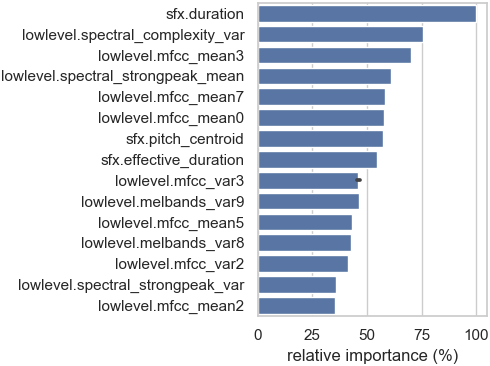
\includegraphics[width=\columnwidth]{Figures/SELD/importance_new_tight.png}}
  \caption{Most representative features in event classifier.}
  \label{fig:importance}
\end{figure}

Fig.~\ref{fig:importance} shows the relative importance of the fifteen most relevant acoustic features for the \textit{PAPAFIL2} classifier model.
Event duration is clearly the feature with the highest importance, and effective duration (duration of the signal discarding silence) also appears in the eighth position.
This fact can help to explain the better performance of \textit{PAPAFIL2} over \textit{PAPAFIL1}: the temporal activities of the events in training and prediction are much more similar to each other in the former method, as a consequence of the training set generation approach. 
In order to provide a deeper insight on the temporal characteristics of the data under consideration, the durations of all sound events in the \textit{PAPAFIL2} training set are summarized in Figure~\ref{fig:eventdurations}. \\

\begin{figure}[t]
  \centering
  \centerline{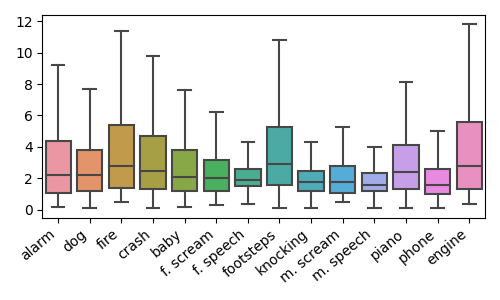
\includegraphics[width=\columnwidth]{Figures/SELD/event_durations.png}}
  \caption{Event durations of all elements in the \textit{PAPAFIL2} training set.}
  \label{fig:eventdurations}
\end{figure}


Furthermore, it is interesting to notice the high relevance of low-level features; specifically, several MFCC combinations (eight of the fifteen reported features) and various extractors related to the spectral structure. The absence of pitch, harmonic and envelope features in the list represents also a significant finding. \\



The results of the DCASE 2020 Challenge for the SELD task are shown in Table~\ref{tab:dcase2020results}. The method entries corresponds to the best scoring method for each team submission, respecting the naming conventions established for the Challenge. Accordingly, \textit{PerezLopez} refers there to the \textit{PAPAFIL2} method. 
The final rank is computed as the cumulative rank across all evaluation metrics, sorted by ascending order. The data has been taken from the Task results website \cite{dcasetask}, which provides complete information regarding the challenge.


\begin{table}[t]
\begin{footnotesize}
\caption{DCASE 2020 Challenge Task 3 evaluation results}
    \begin{center}	

\begin{tabular}{llccccc}
    \toprule
Rank       & Method  & $\text{ER}_{20}$ & $\text{F}_{20}$   & $\text{LE}_{CD}$ & $\text{LR}_{CD}$ & $\text{SELD}$ \\
    \midrule
\textbf{1} & Du & \textbf{0.20}  & \textbf{84.9} \%    & \textbf{6.0}$^{\circ}$   & 88.5 \%    &  \textbf{0.12 }    \\
2          & Nguyen          & 0.23  & 82.0 \%    & 9.3$^{\circ}$   &\textbf{ 90.0} \%    &  0.14     \\
3          & Shimada         & 0.25  & 83.2 \%    & 7.0$^{\circ}$   & 86.2 \%    &  0.15     \\
4          & Cao             & 0.36  & 71.2 \%    & 13.3$^{\circ}$  & 81.1 \%    &  0.22     \\
5          & Park            & 0.43  & 65.2 \%    & 16.8$^{\circ}$  & 81.9 \%    &  0.26     \\
6          & Phan            & 0.49  & 61.7 \%    & 15.2$^{\circ}$  & 72.4 \%    &  0.30     \\
7          & PerezLopez      & 0.51  & 60.1 \%    & 12.4$^{\circ}$  & 65.1 \%    &  0.33     \\
8          & Sampathkumar    & 0.53  & 56.6 \%    & 14.8$^{\circ}$  & 66.5 \%    &  0.35     \\
9          & Patel           & 0.55  & 55.5 \%    & 14.4$^{\circ}$  & 65.5 \%    &  0.38     \\
10         & Ronchini        & 0.58  & 50.8 \%    & 16.9$^{\circ}$  & 65.5 \%    &  0.39     \\
11         & Naranjo-Alcazar & 0.61  & 49.1 \%    & 19.5$^{\circ}$  & 67.1 \%    &  0.38     \\
12         & Song            & 0.57  & 50.4 \%    & 20.0$^{\circ}$  & 64.3 \%    &  0.38     \\
13         & Tian            & 0.64  & 47.6 \%    & 24.5$^{\circ}$  & 67.5 \%    &  0.40     \\
14         & Singla          & 0.88  & 18.0 \%    & 53.4$^{\circ}$  & 66.2 \%    &  0.58     \\
15         & Baseline        & 0.69  & 41.3 \%    & 23.1$^{\circ}$  & 62.4 \%    &  0.45     \\
\bottomrule      
\end{tabular}
\end{center}
    \label{tab:dcase2020results}
    \end{footnotesize}
\end{table}

It is important to remark that, apart from our proposed method, all other systems rely completely on deep learning algorithms, specially making use of different configurations and combinations of CRNNs. 

The only exception to that tendency is the method presented by Nguyen and colleagues, which is an adaptation of their recently proposed methodology \cite{Nguyen2020_task3_report, nguyen2020sequence}. In this method, localization is also based on the identification of the single-source TF bins; instead of DirAC diffuseness, they use a subspace analysis to find the TF bins associated with nearly rank-1 spatial covariance matrices. 
Furthermore, the instantaneous DOA estimates are obtained by finding the azimuth and elevation histogram peaks, with the steering directions obtained from the covariance matrix diagonals. \\

While this method might contribute to provide a smaller localization error compared with our approach (9.3$^{\circ}$ versus 14.2$^{\circ}$ in $\text{LE}_{CD}$), it is more expense computationally, since it involves building a SCM for each TF bin, plus peak picking in two 1D histograms (one for each spherical coordinate). 
However, the $\text{LE}_{CD}$ results are also influenced by the classification accuracy; a deeper analysis would be required to perform a direct comparison of both approaches.

Table~\ref{tab:dcase2020results} also highlights the good result obtained by our method regarding localization error: it is the fourth best method with respect to $\text{LE}_{CD}$. 
Moreover, the two model-based localization methods (our system and Nguyen) rank fourth and second in the $\text{LE}_{CD}$ classification, respectively. 
This result suggests that parametric spatial audio analysis, combined with a robust tracking system, is able to produce state-of-the-art localization results in the context of SELD. \\

To conclude the analysis, Figure~\ref{fig:importance} shows the relationship between the system complexity, measured in number of parameters of the model, against $\text{SELD}$ score, for all submitted systems, denoted by their ranking position. 
The overall tendency is clear: the higher the number of parameters, the better (smaller) the $\text{SELD}$ score; the regression curve, computed from all observations, confirms such tendency. 
It must be noticed that the presented method (\textit{7} in the Figure) lies outside the 95\% confidence interval of the regression curve (shaded area). In other words, its $\text{SELD}$ score is significantly better than the tendency observed from all submissions, considering the system complexity. 
Figure~\ref{fig:importance} also highlights the great difference in complexity among submissions. Between our method (the less complex, with 20k parameters) and the first scoring method (the most complex, with 123M parameters) there are four magnitude orders of different, constituting a remarkable difference. The logarithmic mean of all submitted systems' complexities is around 2.3M parameters. 

\begin{figure}[t]
  \centering
  \centerline{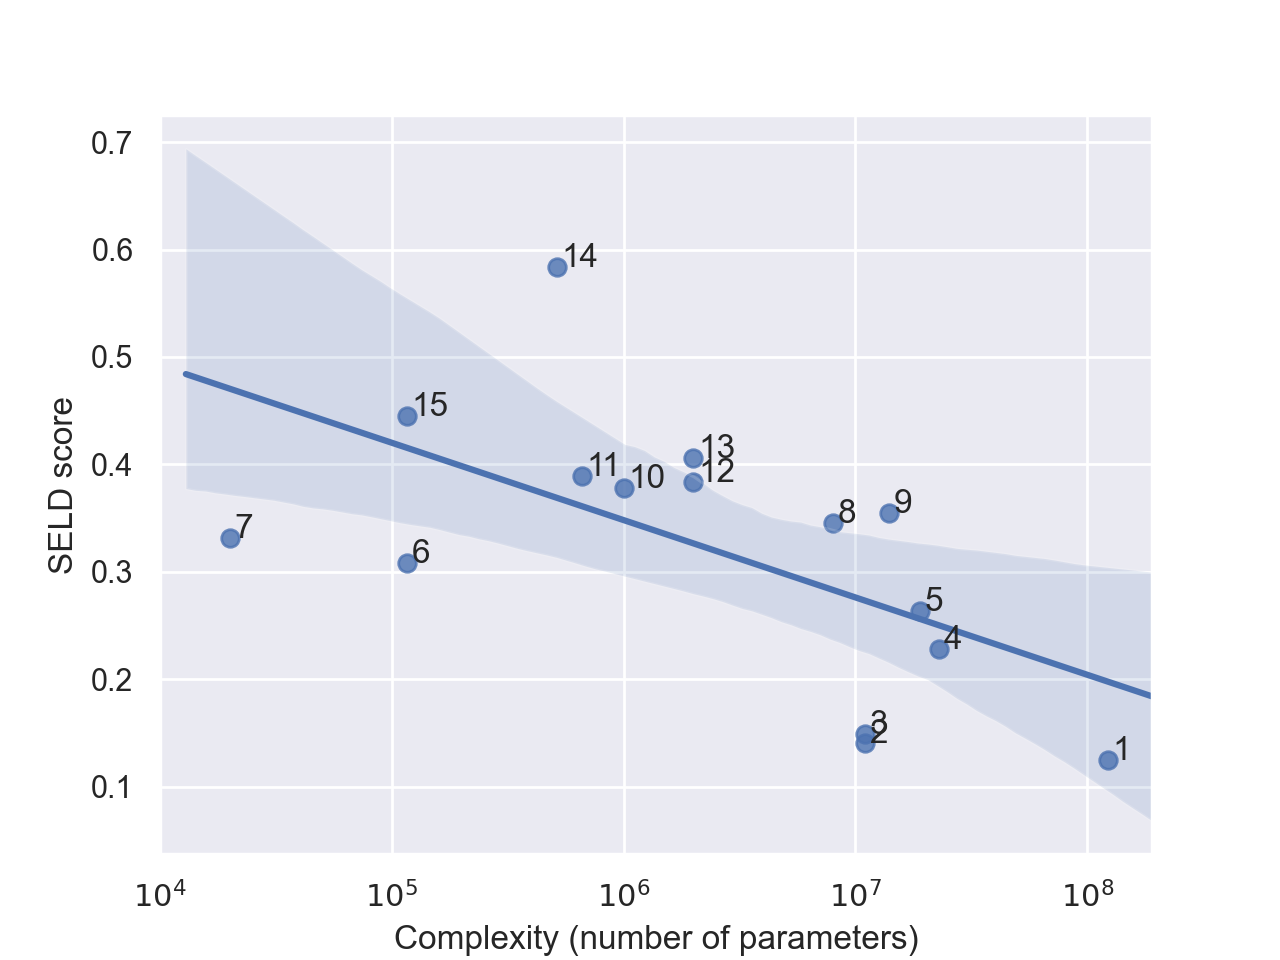
\includegraphics[width=0.8\columnwidth]{Figures/SELD/seld_complexity_v4.png}}
  \caption{DCASE 2020 Task 3 submissions: complexity versus SELD score.}
  \label{fig:importance}
\end{figure}



%%%%%%%%%%%%%%%%%%%%%%%%%%%%%%%%%%%%%%%%%%%%%%%%%%%%%%%%%%%%
%%%%%%%%%%%%%%%%%%%%%%%%%%%%%%%%%%%%%%%%%%%%%%%%%%%%%%%%%%%%
\section{Conclusion}
\label{sec:results}

% We have presented a novel method for Sound Event Localization and Detection (SELD), based on parametric particle filtering and gradient boosting single-class event classification of audio features. Results show that the proposed method outperforms the baseline method, a state-of-the-art Convolutional Recurrent Neural Network (CRNN). Specifically, the proposed method is able to improve the baseline SELD score by almost ten points, while also increasing the evaluation score in three out of the four proposed metrics, by means of a low complexity machine learning architecture.

We present a novel low-complexity method for Sound Event Localization and Detection of First Order Ambisonic signals, based on four steps: estimation of single-source spectrogram regions by parametric analysis; computation of event trajectories and activations by means of a particle tracker; spatio-temporal filtering of the input signal; and single-class monophonic event classification by Gradient Boosting. 
Results show that the proposed method outperforms the baseline method, a state-of-the-art Convolutional Recurrent Neural Network. Specifically, our method is able to improve the baseline SELD score by almost ten points, while increasing the scores in three out of the four metrics under consideration.
